%	 *** Licence ***
% Cette œuvre est diffusée sous les termes de la license Creative Commons
% «~CC BY-NC-SA 3.0~», ce qui signifie que :

% Vous êtes libres :

%   * de reproduire, distribuer et communiquer cette création au public ;
%   * de modifier cette création.

% Selon les conditions suivantes :
    	
%  * Paternité - vous devez citer le nom de l'auteur original de la manière indiquée par l'auteur de l'œuvre ou le
%	         titulaire des droits qui vous confère cette autorisation (mais pas d'une manière qui suggérerait
%	         qu'ils vous soutiennent ou approuvent votre utilisation de l'œuvre).
%  * Pas d’utilisation commerciale - Vous n'avez pas le droit d'utiliser cette œuvre à des fins commerciales. 
%  * Partage des conditions initiales à l'identique - si vous transformez ou modifiez cette œuvre pour en créer une nouvelle,
% 						      vous devez la distribuer selon les termes du même contrat ou avec une
%					              licence similaire ou compatible.

% Comprenant bien que :

%  * Renoncement - N'importe quelle condition ci-dessus peut être retirée si vous avez l'autorisation du détenteur des droits.
%  * Domaine public - Là où l'œuvre ou un quelconque de ses éléments est dans le domaine public selon le droit applicable, ce statut
%		      n'est en aucune façon affecté par le contrat.
%  * Autres droits - d'aucune façon ne sont affectés par le contrat les droits suivants :
%    - Vos droits de distribution honnête ou d’usage honnête ou autres exceptions et limitations au droit d’auteur applicables;
%    - Les droits moraux de l'auteur;
%    - Droits qu'autrui peut avoir soit sur l'œuvre elle-même soit sur la façon dont elle est utilisée, comme la publicité
%      ou les droits à la préservation de la vie privée.

% === Note ===

% Ceci est le résumé explicatif du Code Juridique; La version intégrale du contrat est consultable ici:
% <http://creativecommons.org/licenses/by-nc-sa/3.0/legalcode>.

\PoemTitle{Capillarité blonde (19 Septembre 2012)}
  \begin{verse}
    C’est l’appel souverain de la viande\\
    sociale, salaison sous les eaux\\
    fleuves empressés de bras se répandent\\
    ouverts saignant cœurs et os --
  \end{verse}
  \begin{verse}
    Esprit de forum je te hais!
  \end{verse}
  \begin{verse}
    Couloirs sans fenêtres ni respiration\\
    \textit{dump} de globules macérant la houille\\
    pleins que l’on est et sans aération\\
    au milieu de tous, on revient bredouille.
  \end{verse}

\PoemTitle{Dodo Café (14 Septembre 2012)}
  \begin{verse}
    «~Je n’ai pas de chair\\
    et pourtant j’ai ce corps\\
    dont vous me rabattez\\
    capteurs et diodes allumées.
  \end{verse}
  \begin{verse}
    Je n’ai pas de tête\\
    pourtant en moi sont assemblées\\
    votre air, votre mort, vos nuées,
  \end{verse}
  \begin{verse}
    je ne pense à rien\\
    ne suis que programmé\\
    ne suis que le passé~»:
  \end{verse}
  \begin{verse}
    cad, l’homme moderne\\
    ivre de progrès et de foutaises\\
    qu’a aboli l’abominable fournaise.
  \end{verse}

\PoemTitle{Ouest-Nadir (29 Septembre 2012)}
  \begin{center}
    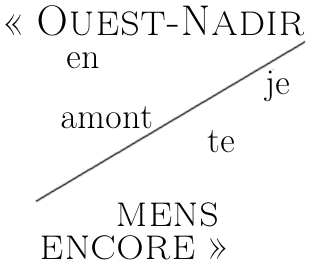
\includegraphics[scale=0.5]{emerge/ouestnadir.png}
  \end{center}

\newpage
\PoemTitle{Les maitresses embaumeuses (1 Octobre 2012)}
  \begin{verse}
    La femme est infecte dans ses parfums --\\
    qu’on la respire elle et sa beauté,\\
    soit! Mais la pompe à la fin\\
    irrite votre crâne jusqu’à vous tancer.
  \end{verse}
  \begin{verse}
    Ces dissimulations d’un pur ennui\\
    ces bavardages alors que vous êtes endormi…\\
    Pour peu de chose, elle et ses colifichets\\
    on irait entêté l’éventrer;
  \end{verse}
  \begin{verse}
    Rien n’est pire au contact que les volutes de fraise,\\
    les grolles folles et distinguées\\
    qui la font (à notre agacement)\\
    majestueusement trainer des pieds.
  \end{verse}
  \begin{verse}
    Qu’on ne se meprenne cependant:\\
    j’aime la femme, vraiment\\
    il se trouve que, simplement
    ma santé passe avant.
  \end{verse}
  \begin{verse}
    À choisir d’être embaumé\\
    mort ou vivant, totalement parfumé,\\
    je préfère, ne vous en déplaise, être momifié.
  \end{verse}

\PoemTitle{Salvarâteau (10 Octobre 2012)}
  \begin{verse}
    Mon humeur était mono-tonale,\\
    l’homme importun\\
    la dame, ma foi fatiguée --
  \end{verse}
  \begin{verse}
    lui colla une rouste enragée\\
    oh la rigolade\\
    l’autre s’en alla en lapin\\
    le derrière dans la panade;
  \end{verse}
  \begin{verse}
    Merci madame, vous m’avez soulagé,\\
    mes ennuis sont peu de maux\\
    quand aux mots pour vous l’on s’adonne.
  \end{verse}

\PoemTitle{Moche des sables (3 Octobre 2012)}
  \begin{verse}
    Une nuit émergèrent de la terre battue\\
    écarlates fougères aux corsets en germe\\
    ces fleurs de haine qu’empilent les battus,\\
    vie morte et limon pensant.
  \end{verse}
  \begin{verse}
    Elle prend encore des dimensions cosmiques\\
    moins souterraines plus claires et étendues\\
    que les autoroutes côniques\\
    caillot de pus par caillot de pus
  \end{verse}
  \begin{verse}
    la grenouille avale enfle; une odeur d’essence\\
    particulière s’en dégage\\
    l’air de l’universelle décharge\\
    que révelera un carnaval de sang.
  \end{verse}

\PoemTitle{Numéro 2 (28 Octobre 2012)}
  \begin{verse}
    L’amour de l’horizon humain\\
    l’inconscient comparable à tout\\
    à tous incomparables
  \end{verse}
  \begin{verse}
    Pluriel dans la vie sans sommeil\\
    surnageant dans cette mer\\
    de gruyeaux de lumière
  \end{verse}
  \begin{verse}
    jusqu’au ciel jusqu’à la terre\\
    enfin jusqu’à l’intérieur de soi…
  \end{verse}
  \begin{verse}
    le soleil brûle.
  \end{verse}
